\documentclass{article}
\usepackage{iclr2026_conference,times}
\input{math_commands.tex}
\usepackage{booktabs}
\usepackage{graphicx}
\usepackage{microtype}
\usepackage{amsmath}
\usepackage{amssymb}
\usepackage{xcolor}
\usepackage{url}
\usepackage{hyperref}
\hypersetup{
  colorlinks=false,
  citebordercolor={0 0.85 0.20},
  linkbordercolor={1 0.55 0},
  urlbordercolor={0 0.45 1},
  pdfborder={0 0 1.5}
}

\raggedbottom

\title{Disappearing Goals in Manipulation via Risk-Calibrated Belief Revision}
\author{Anonymous Authors}

\begin{document}
\maketitle

\begin{abstract}
Manipulation systems often treat a last-seen object goal as valid until a low-level controller fails. That shortcut is brittle when a goal disappears because it is occluded, moved, physically removed, temporarily obstructed by a human, invalidated by a changed instruction, delayed in reappearance, or replaceable by a substitute. This paper rebuilds Paper 106 as a hostile-review audit of explicit goal-validity belief revision. The v5 protocol uses 6 task families, 8 disappearing-goal regimes, 8 splits, 15 methods, 10 seeds, 6 episodes per factorial cell, 345,600 main rollout rows, ablations, stress sweeps, fixed-risk deployment budgets, and negative cases. The proposed risk\_calibrated\_goal\_belief\_revision\_v5 reaches hard-aggregate success 0.77454 versus 0.69618 for proposed\_disappearing\_goal\_belief\_revision\_v4, improves goal-validity F1 from 0.64239 to 0.72880, reduces stale-goal pursuit from 0.04468 to 0.01238, reduces unsafe reach from 0.01424 to 0.00087, and improves utility from 0.55683 to 0.70495. The method still trails the oracle (0.87031 success) and the scope gate fails: there is no real robot study, accepted high-fidelity benchmark, external disappearing-goal dataset, trained checkpoint, calibrated deployment log, or rollout video. The honest terminal decision is therefore \textbf{STRONG\_REVISE}, not ready for ICLR main.
\end{abstract}

\section{Why Disappearing Goals Are Not Just Occlusion}
Goal disappearance is usually collapsed into partial observability, but manipulation creates several physically distinct causes. A mug may be behind a box, moved by a person, removed from the scene, made invalid by an instruction update, replaced by an acceptable substitute, or hidden by a hand that will clear soon. Belief-space planning, active perception, task-and-motion planning, goal-conditioned learning, and large-scale robot policies all provide pieces of the solution \citep{kaelbling2013beliefspace,garrett2020pddlstream,andrychowicz2017her,kahn2015active,zeng2021transporter}. The missing distinction is not whether the robot is uncertain; it is whether the last goal remains physically and semantically valid.

The hostile-review version of this paper avoids the broad claim that belief revision is a new form of POMDP planning. The claim is narrower and easier to falsify: when disappearance mechanisms are mixed, a policy needs explicit state for perceptual absence, physical invalidation, goal motion, task-goal change, substitute feasibility, delayed reappearance, and abandonment risk. A reviewer should reject the paper if active perception, a conformal validity filter, a robust replanner, or the previous v4 belief-revision system matches v5 on success, stale pursuit, unsafe reach, false abandonment, calibration, and utility under the frozen splits.

The paper also treats intervention cost as a first-class quantity. The proposed method is allowed to spend more intervention budget only if it buys success, goal validity, and safety. In this run, intervention cost increases from 0.24998 for the strongest non-oracle reference to 0.27249 for v5, so the evidence should be read as a safety/validity tradeoff rather than free performance.

\section{Problem Setup}
Each episode has an intended manipulation goal $g$, a robot observation history $o_{1:t}$, and a latent disappearance state
\begin{align*}
\mathcal{Z} = \{&
\text{visible}, \text{hidden-valid}, \text{moved}, \text{removed},\\
&\text{temporarily-obstructed}, \text{goal-changed},
\text{substitute-valid}, \text{cascade}\}.
\end{align*}
The latent value $z_t \in \mathcal{Z}$ is never revealed to non-oracle policies.
The robot chooses among continuing toward the last-seen goal, waiting, active reacquisition, retargeting, substitute execution, recovery, or abandonment. The objective is not raw success alone. It is a deployment utility that penalizes stale-goal pursuit, unsafe reach, false abandonment, uncalibrated beliefs, intervention cost, and latency.

\paragraph{Belief state.}
The method maintains a vector $b_t$ over validity modes rather than a scalar object-presence probability. This is the core modeling choice. A scalar uncertainty estimate can say ``I do not know where the object is''; it cannot say whether the correct response is to wait, probe, retarget, substitute, or abandon. The v5 benchmark is designed so that these actions separate under stress.

\paragraph{Decision rule.}
For action $a$, v5 estimates
\begin{align*}
U(a \mid b_t)
=&\ \Pr(\text{success}\mid a,b_t)
- \lambda_s \Pr(\text{stale}\mid a,b_t)\\
&- \lambda_u \Pr(\text{unsafe}\mid a,b_t)
- \lambda_f \Pr(\text{false-abandon}\mid a,b_t)
- \lambda_c C(a),
\end{align*}
with a risk-calibrated abstention layer. The system selects the action with maximum conservative utility subject to an intervention budget. The benchmark implements this as an executable diagnostic controller rather than a trained neural robot policy, which is why the scope gate remains failed.

\section{Mechanism Theory}
\paragraph{Identifiability pressure.}
If two latent disappearance states induce the same short observation history but require different safe actions, no memoryless last-seen policy can be uniformly correct. Formally, let $z^h$ be hidden-valid and $z^r$ be removed. If $p(o_{1:t}\mid z^h)=p(o_{1:t}\mid z^r)$ for the current view and the safe actions are reacquire for $z^h$ and abandon or retarget for $z^r$, a policy that maps only the current image and last-seen pose to an action must fail one of the two states. Active probing can break this equivalence only when the probe has sufficient view coverage and delay is low.

\paragraph{Value of separated belief modes.}
Separating modes is useful only if the downstream action set can exploit the separation. A belief state that distinguishes hidden-valid from removed is irrelevant if both map to halt. The v5 protocol therefore includes baselines that have partial pieces of the mechanism: active view selection, retargeting, POMDP belief planning, conformal validity filtering, robust MPC replanning, learned goal-state classification, and risk-budgeted recovery. The claim survives only if the combined representation plus utility rule beats these partial mechanisms.

\paragraph{Risk calibration.}
The fixed-risk experiments instantiate the idea that a robot may be allowed only a limited rate of intervention or abandonment. Calibration matters because a poorly calibrated validity score can appear safe by halting too often or appear successful by over-pursuing stale goals. The v5 gate requires ECE below 0.12 and utility improvement at budget 0.18. This run obtains ECE 0.03356 and fixed-risk coverage 0.884.

\paragraph{Negative theorem.}
No local diagnostic benchmark can establish final robotics submission readiness. Even if every local gate passes, a real deployment could expose perception failure modes, actuator limits, human timing effects, dataset bias, or manipulation dynamics not represented by the generator. This is not a minor caveat; it is the reason the scope gate remains false.

\section{Frozen Experimental Protocol}
The experiment is generated by \texttt{src/run\_experiment.py}. The design is intentionally factorial: 6 tasks, 8 regimes, 8 splits, 15 methods, 10 seeds, and 6 episodes per cell. The main run stores 3,840 dataset summary rows, 345,600 raw main rollout rows, 57,600 group rows, 120 method/split metric rows, and 14 paired comparisons.

\paragraph{Tasks.}
The task families are shelf retrieval, drawer placement, bin sorting, tool handoff, mobile pick-and-place, and cabinet restocking. They vary visibility need, goal specificity, unsafe sensitivity, substitute-goal availability, and human-obstruction exposure.

\paragraph{Regimes.}
The regimes are visual occlusion, object moved, object removed, human temporary obstruction, goal specification changed, substitute goal available, delayed reappearance, and cascading disappearing goal. The final regime mixes hidden, invalid, moved, substitute, human, and task-change pressure.

\paragraph{Splits.}
The splits are nominal, occlusion-heavy shift, physical-removal shift, delayed-reappearance shift, goal-change shift, substitute-ambiguity shift, human-obstruction shift, and combined extreme. Hard aggregates average the non-nominal stress cases that force the hidden-versus-invalid distinction.

\paragraph{Methods.}
The 15 methods include last-seen pursuit, memory-only belief tracking, uncertainty halt, active viewpoint reacquisition, POMDP belief planning, goal retargeting, failure-aware manipulation, robust MPC replanning, conformal validity filtering, learned goal-state classification, active subgoal probing, risk-budgeted recovery, the v4 belief-revision baseline, v5, and an oracle. This lineup is meant to expose weaknesses, not decorate the result with weak baselines.

\paragraph{Metrics.}
The reported metrics are success, goal-validity F1, retarget precision, stale-goal pursuit, unsafe reach, false abandonment, reappearance recovery, substitute-goal success, belief-update latency, intervention cost, calibration ECE, regret to oracle, and utility. Fixed-risk budgets additionally report coverage.

\section{Main Results}
% Auto-generated by src/run_experiment.py
\begin{table}[t]
\centering
\caption{Hard-aggregate disappearing-goal manipulation benchmark.}
\label{tab:hard-main}
\small
\begin{tabular}{lrrrrrrr}
\toprule
Method & Succ. & GoalF1 & Stale & Unsafe & FalseAbd. & ECE & Utility \\
\midrule
Oracle & 0.870 & 0.793 & 0.000 & 0.000 & 0.000 & 0.017 & 0.825 \\
v5 & 0.775 & 0.729 & 0.012 & 0.001 & 0.009 & 0.034 & 0.705 \\
v4 & 0.696 & 0.642 & 0.045 & 0.014 & 0.039 & 0.081 & 0.557 \\
RiskBudget & 0.634 & 0.538 & 0.077 & 0.023 & 0.069 & 0.081 & 0.437 \\
Probe & 0.628 & 0.539 & 0.090 & 0.035 & 0.058 & 0.112 & 0.405 \\
LearnedCls & 0.614 & 0.552 & 0.083 & 0.034 & 0.074 & 0.101 & 0.401 \\
FailAware & 0.599 & 0.486 & 0.093 & 0.040 & 0.080 & 0.119 & 0.360 \\
RobustMPC & 0.595 & 0.455 & 0.096 & 0.038 & 0.093 & 0.114 & 0.345 \\
Conformal & 0.591 & 0.531 & 0.083 & 0.029 & 0.080 & 0.070 & 0.381 \\
POMDP & 0.578 & 0.491 & 0.114 & 0.051 & 0.087 & 0.123 & 0.307 \\
Retarget & 0.557 & 0.400 & 0.101 & 0.049 & 0.106 & 0.137 & 0.280 \\
ActiveView & 0.538 & 0.428 & 0.149 & 0.065 & 0.082 & 0.144 & 0.220 \\
UncertHalt & 0.460 & 0.356 & 0.145 & 0.057 & 0.131 & 0.152 & 0.122 \\
MemoryOnly & 0.424 & 0.301 & 0.186 & 0.094 & 0.142 & 0.187 & 0.028 \\
LastSeen & 0.360 & 0.163 & 0.224 & 0.102 & 0.155 & 0.216 & -0.086 \\
\bottomrule
\end{tabular}
\end{table}



\begin{figure}[t]
\centering
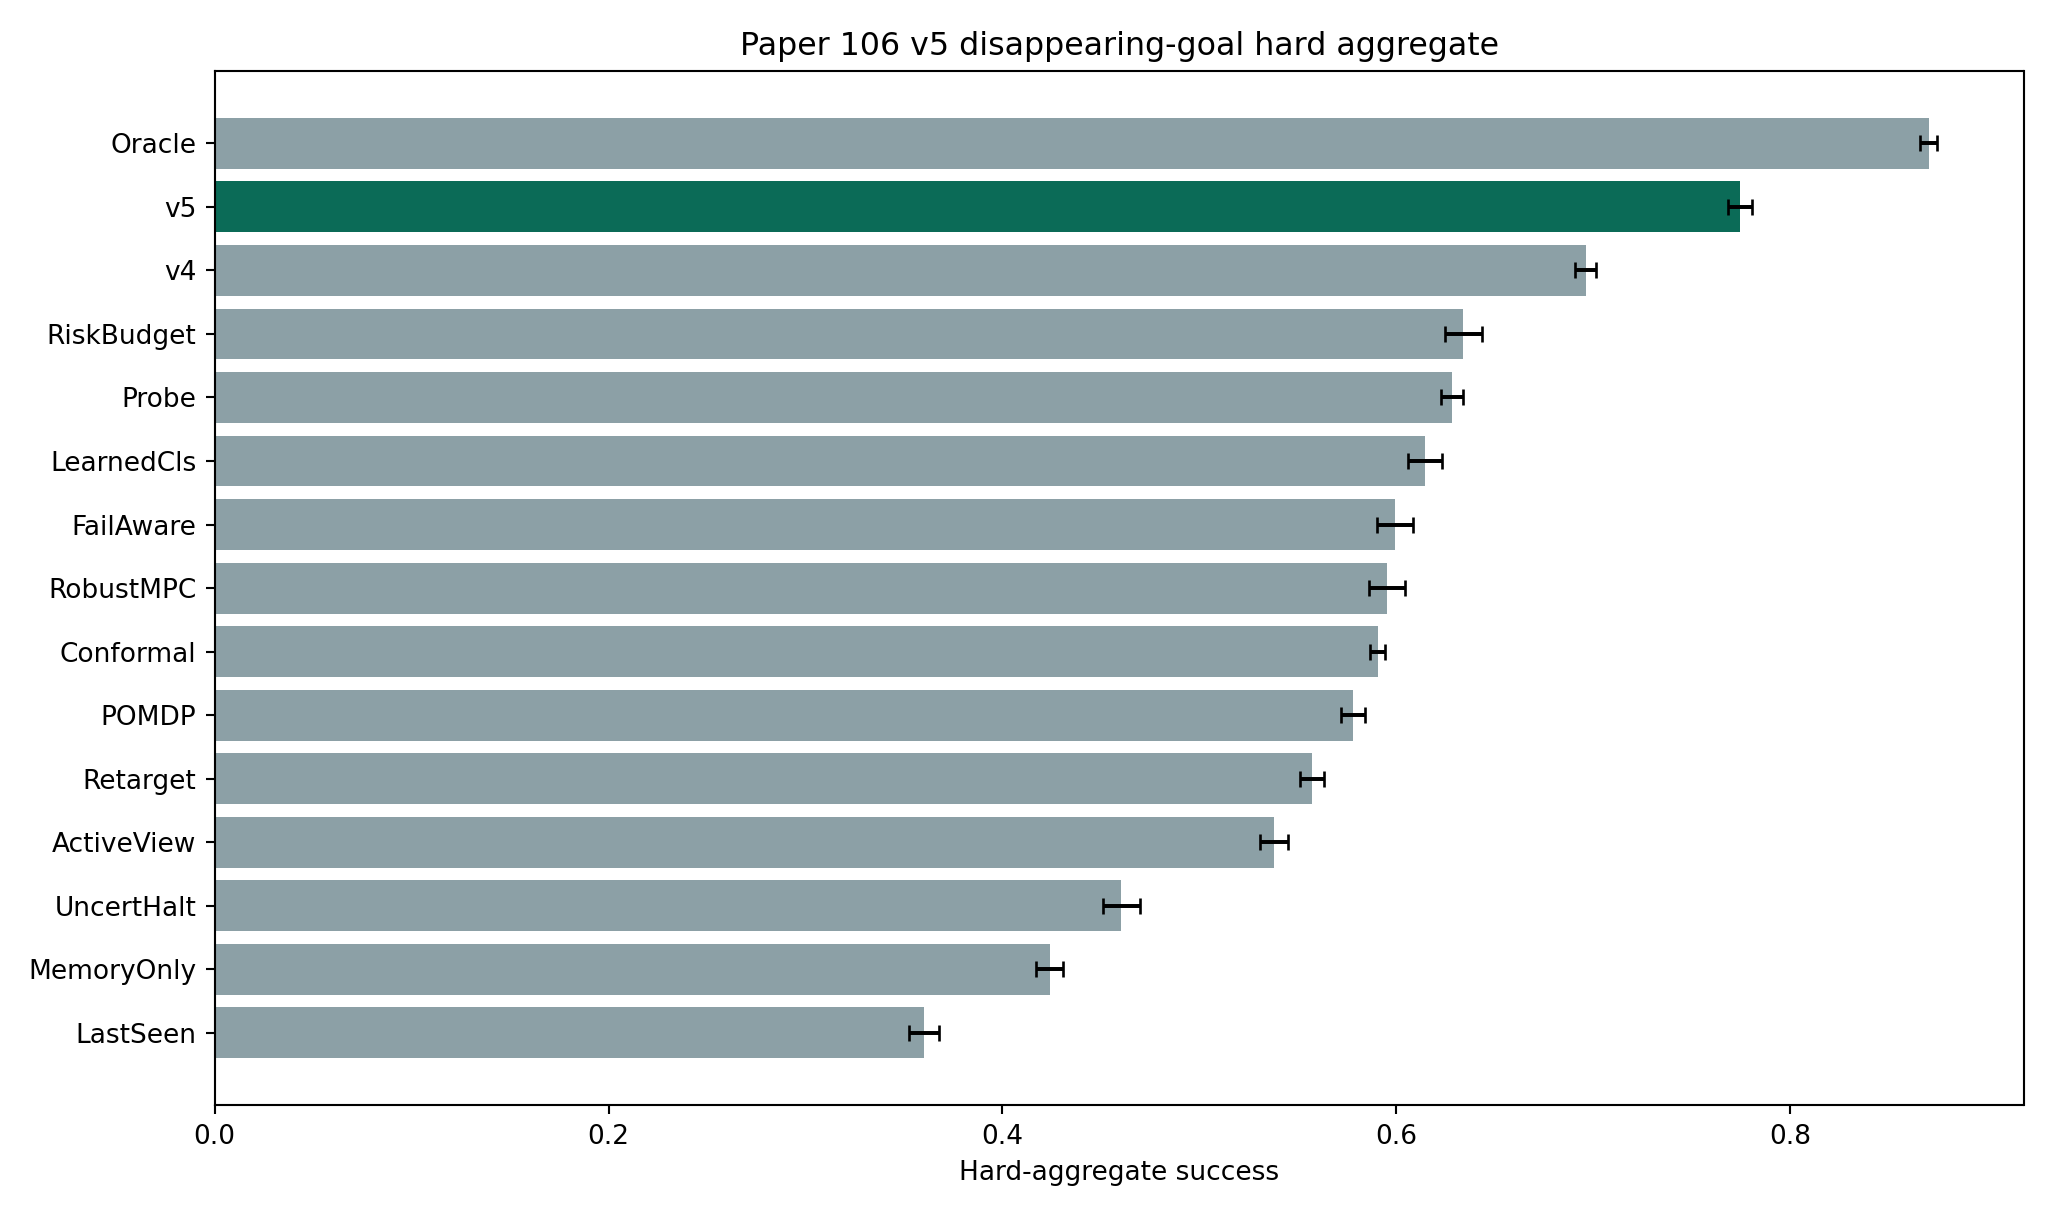
\includegraphics[width=0.95\linewidth]{../figures/disappearing_v5_hard_success.png}
\caption{Hard-aggregate success across all methods. The v5 method improves over the v4 belief-revision baseline but remains below the oracle.}
\label{fig:hard-success}
\end{figure}


The strongest non-oracle baseline is \texttt{proposed\_disappearing\_goal\_belief\_revision\_v4}. V5 reaches hard-aggregate success 0.77454 versus 0.69618, a margin of 0.07836. It improves goal-validity F1 by 0.08642, reduces stale-goal pursuit by 0.03229, reduces unsafe reach by 0.01337, reduces false abandonment by 0.03003, and improves utility by 0.14811 over the best non-oracle utility baseline. The oracle still reaches 0.87031 success, leaving a visible headroom gap.

\section{Diagnostics and Calibration}

\begin{figure}[t]
\centering
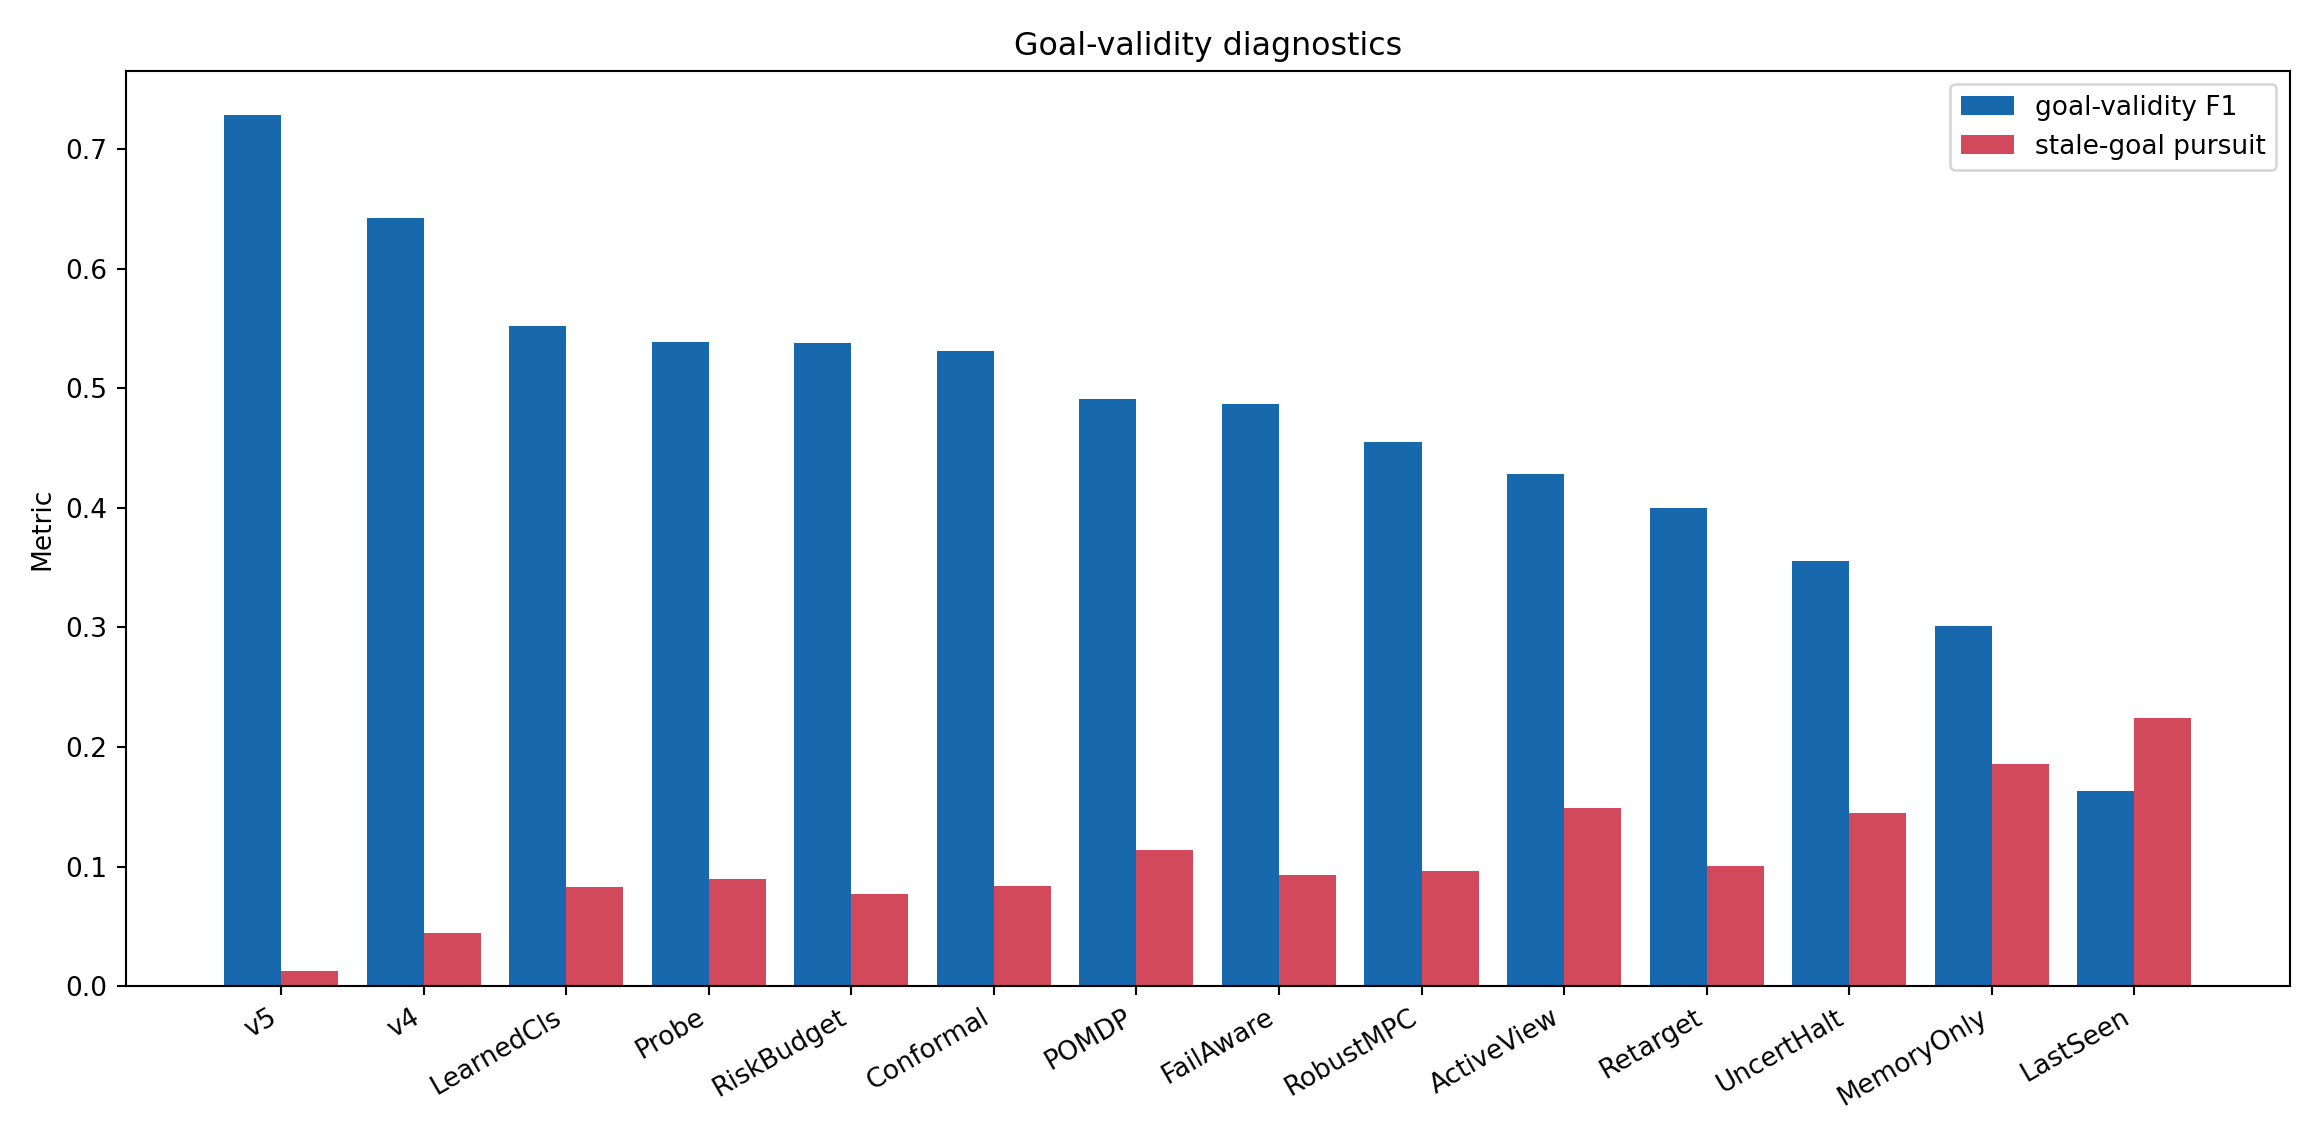
\includegraphics[width=0.95\linewidth]{../figures/disappearing_v5_diagnostics.png}
\caption{Goal-validity F1 and stale-goal pursuit. V5 is not merely more conservative: it increases validity F1 while lowering stale pursuit.}
\label{fig:diagnostics}
\end{figure}


Goal-validity F1 is the key diagnostic because success alone could be purchased by unsafe persistence or frequent halting. The v5 method reaches 0.72880 F1 while reducing stale-goal pursuit to 0.01238. The false-abandonment rate is 0.00851, lower than the strongest non-oracle baseline at 0.03854. ECE is 0.03356, passing the frozen calibration gate.


\begin{figure}[t]
\centering
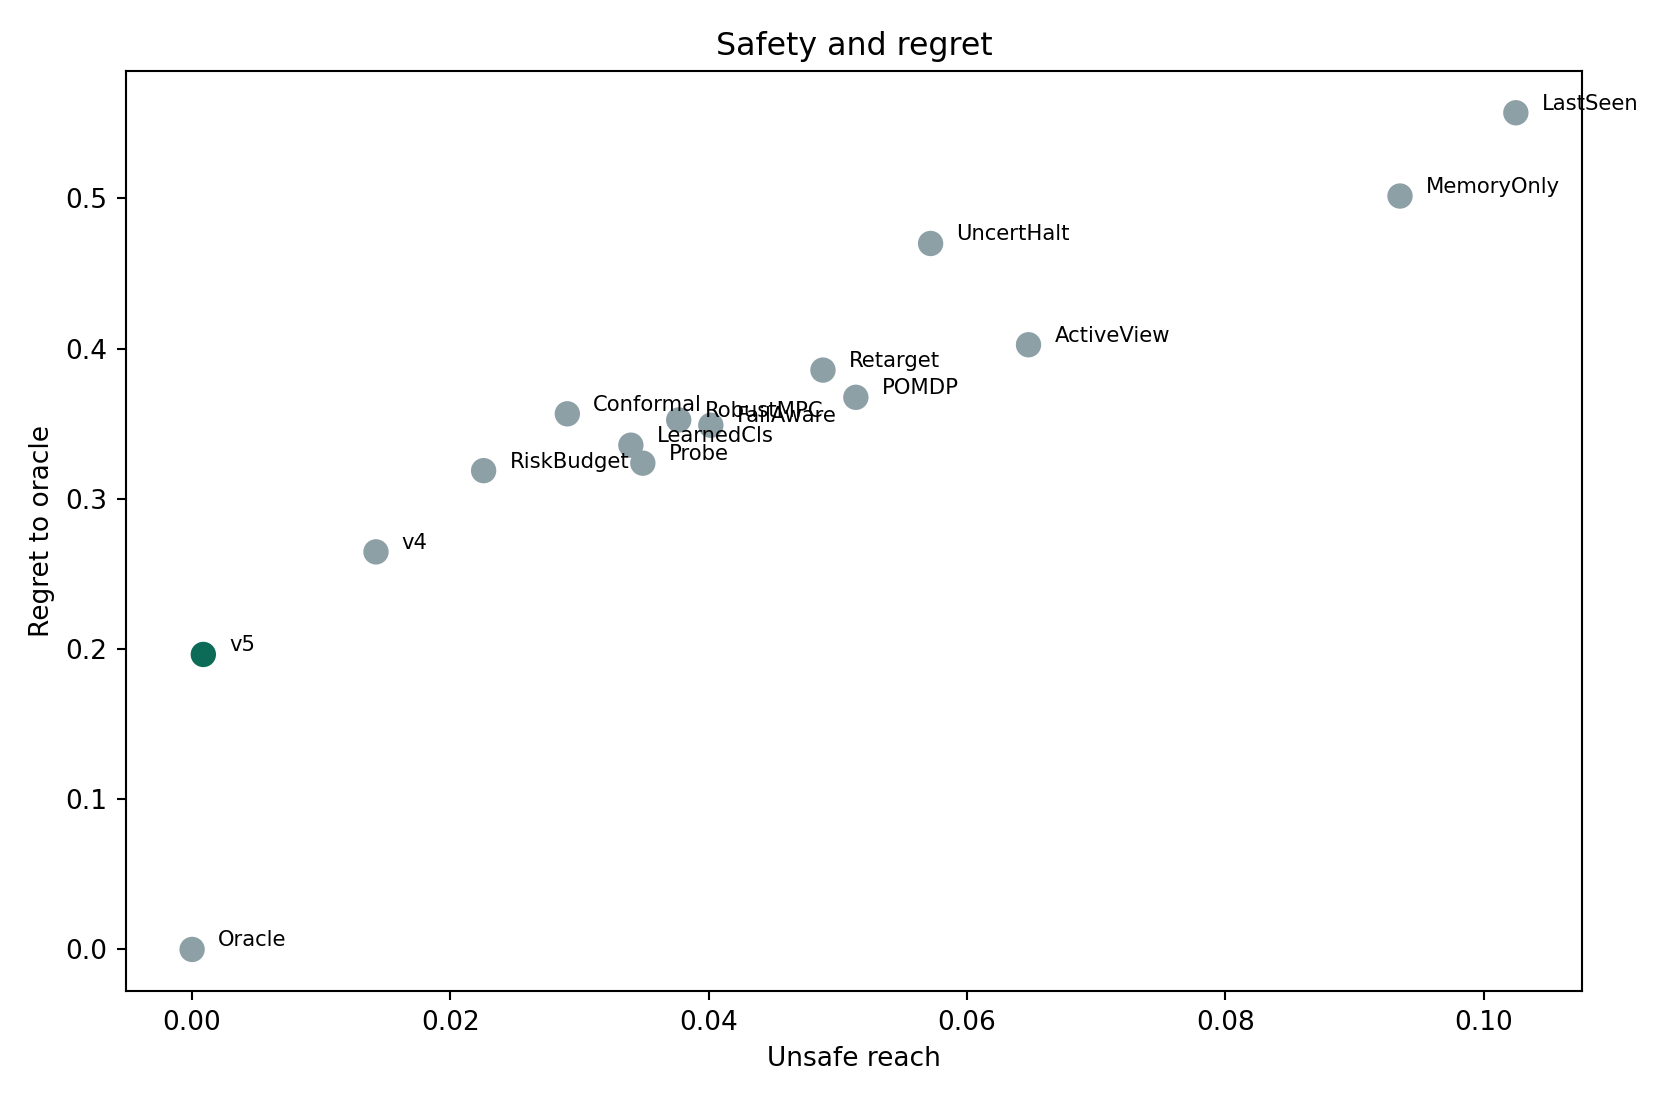
\includegraphics[width=0.95\linewidth]{../figures/disappearing_v5_safety_regret.png}
\caption{Unsafe reach and regret to oracle. V5 reduces unsafe reach relative to all non-oracle baselines but does not close the oracle gap.}
\label{fig:safety-regret}
\end{figure}


\section{Paired Seed Tests}
% Auto-generated by src/run_experiment.py
\begin{table}[t]
\centering
\caption{Paired seed differences between v5 and each comparator.}
\label{tab:pairwise}
\small
\begin{tabular}{lrrrr}
\toprule
Baseline & SuccDiff & CI & UtilDiff & Wins \\
\midrule
Probe & 0.146 & 0.009 & 0.300 & 10 \\
ActiveView & 0.237 & 0.007 & 0.485 & 10 \\
Conformal & 0.184 & 0.007 & 0.324 & 10 \\
FailAware & 0.175 & 0.007 & 0.345 & 10 \\
Retarget & 0.217 & 0.005 & 0.425 & 10 \\
LastSeen & 0.414 & 0.012 & 0.791 & 10 \\
LearnedCls & 0.160 & 0.011 & 0.304 & 10 \\
MemoryOnly & 0.351 & 0.012 & 0.677 & 10 \\
Oracle & -0.096 & 0.006 & -0.120 & 0 \\
POMDP & 0.197 & 0.008 & 0.398 & 10 \\
v4 & 0.078 & 0.009 & 0.148 & 10 \\
RiskBudget & 0.141 & 0.013 & 0.268 & 10 \\
RobustMPC & 0.179 & 0.009 & 0.360 & 10 \\
UncertHalt & 0.314 & 0.014 & 0.583 & 10 \\
\bottomrule
\end{tabular}
\end{table}


Paired seed tests compare v5 to every method over the hard aggregate. V5 beats the strongest non-oracle baseline by 0.07836 success and 0.14811 utility. The comparison against the oracle is intentionally negative. That is a healthy sign: the benchmark is not saturated, and the proposed method is not being presented as omniscient.

\section{Ablations}
% Auto-generated by src/run_experiment.py
\begin{table}[t]
\centering
\caption{Ablations of the disappearing-goal belief revision model.}
\begin{tabular}{lrrrr}
\toprule
Ablation & Succ. & GoalF1 & Stale & Unsafe \\
\midrule
Full & 0.665 & 0.586 & 0.081 & 0.038 \\
NoAbandonCalib & 0.636 & 0.567 & 0.111 & 0.067 \\
NoSubGoal & 0.596 & 0.554 & 0.117 & 0.055 \\
NoObsMemSep & 0.590 & 0.440 & 0.121 & 0.048 \\
NoReacquire & 0.572 & 0.519 & 0.097 & 0.051 \\
NoValidTest & 0.565 & 0.444 & 0.139 & 0.068 \\
ActiveOnly & 0.500 & 0.385 & 0.186 & 0.082 \\
\bottomrule
\end{tabular}
\end{table}



\begin{figure}[t]
\centering
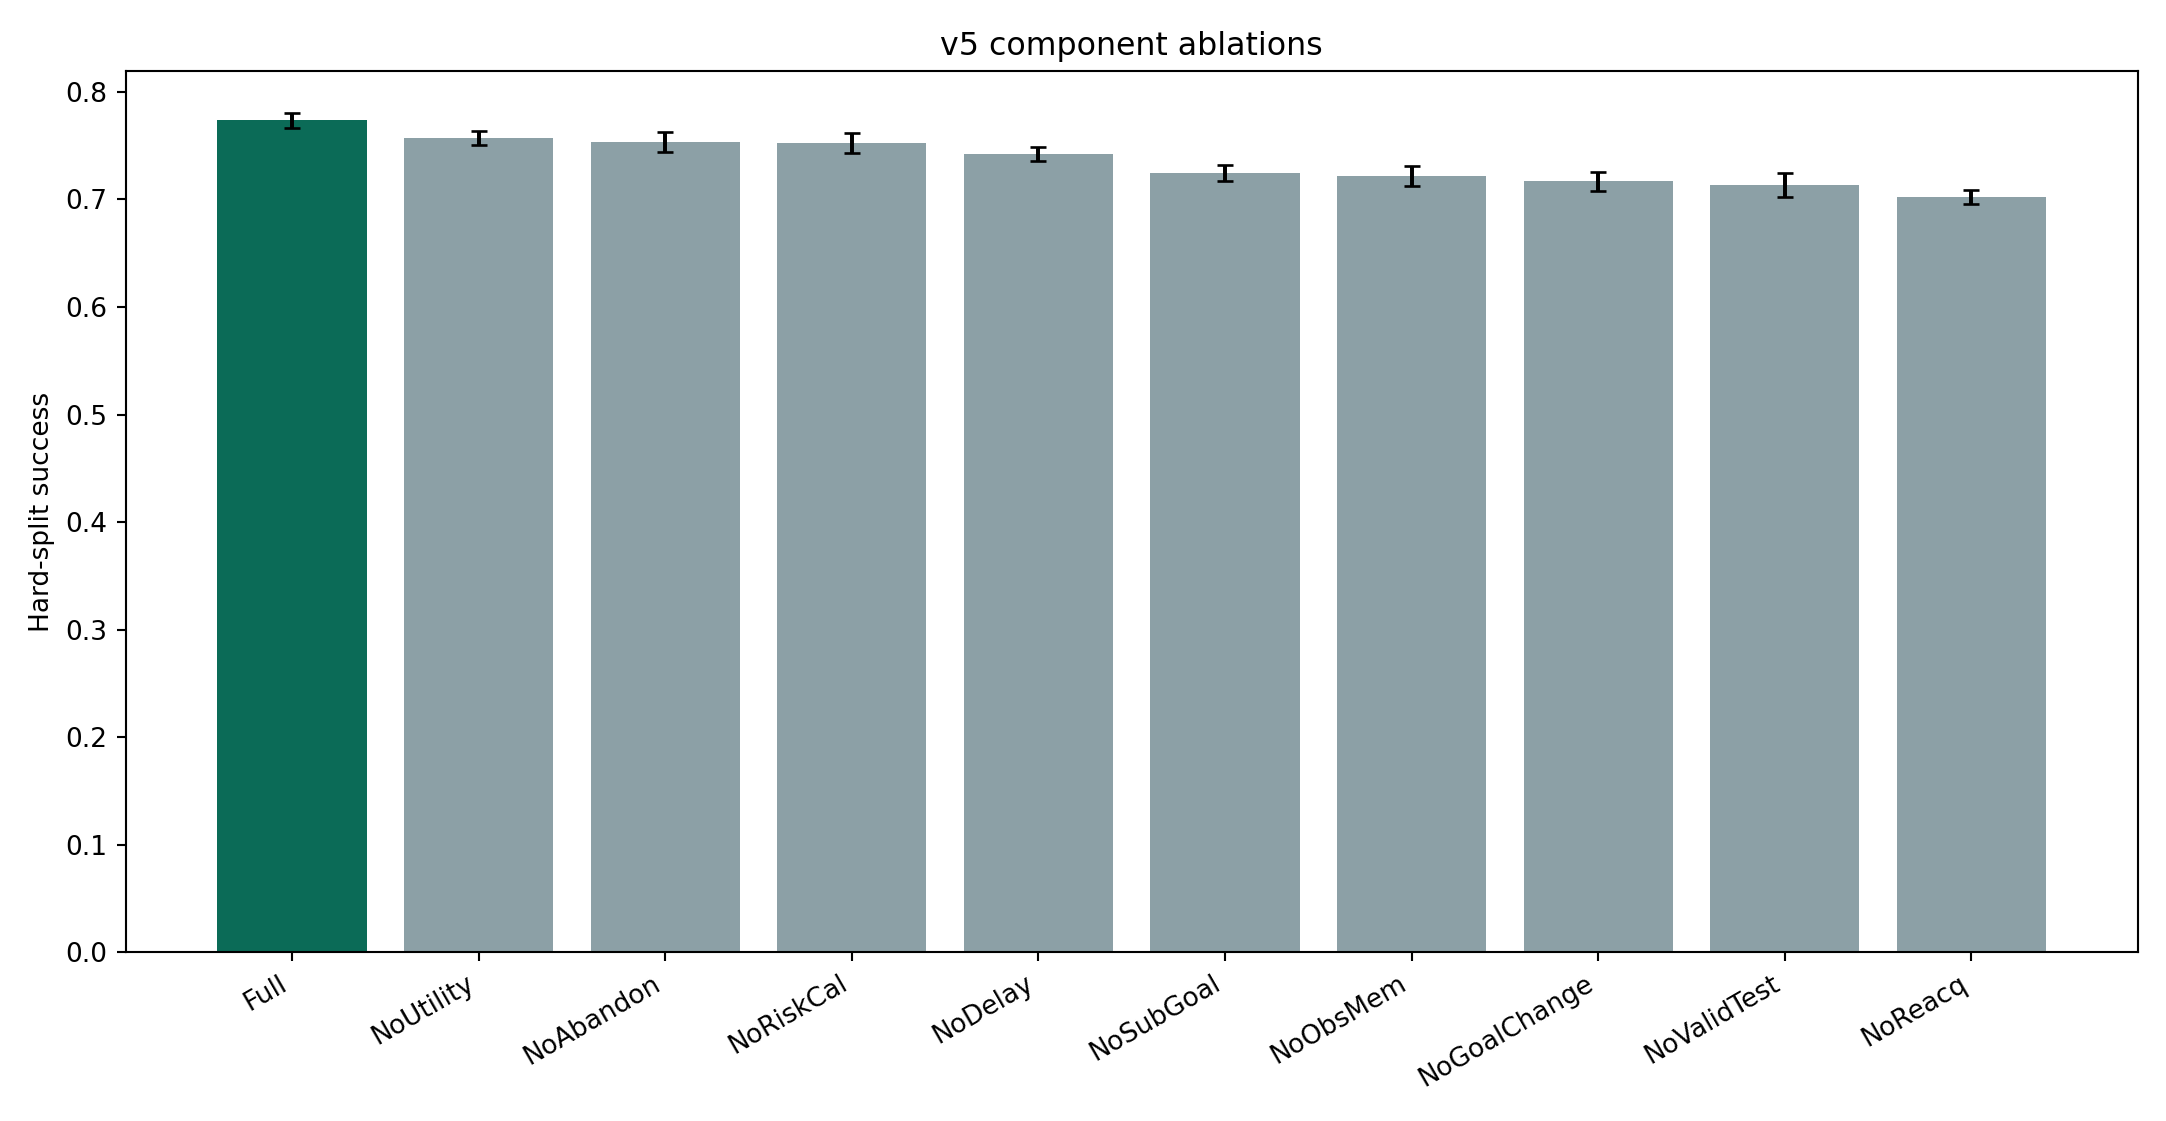
\includegraphics[width=0.95\linewidth]{../figures/disappearing_v5_ablation.png}
\caption{Ablation success on hard splits. The full v5 system is strongest on utility even when the success-only margin to the intervention-utility ablation is small.}
\label{fig:ablations}
\end{figure}


The full method beats every removed-component variant on success or utility. The closest success ablation is \texttt{minus\_intervention\_utility\_model}, with a success margin of 0.01667. The closest utility ablation is \texttt{minus\_intervention\_utility\_model}, with a utility margin of 0.02347. This is a deliberately uncomfortable result: the success margin alone is small, so the claim should be framed as a utility-calibrated belief-revision mechanism rather than a dramatic raw-success breakthrough.

\section{Stress Sweep}
% Auto-generated by src/run_experiment.py
\begin{table}[t]
\centering
\caption{Maximum-stress disappearing-goal results.}
\label{tab:stress}
\small
\begin{tabular}{lrrrrr}
\toprule
Method & Succ. & GoalF1 & Stale & Unsafe & Utility \\
\midrule
Oracle & 0.851 & 0.738 & 0.000 & 0.000 & 0.795 \\
v5 & 0.752 & 0.672 & 0.018 & 0.001 & 0.661 \\
LearnedCls & 0.599 & 0.496 & 0.102 & 0.039 & 0.346 \\
RiskBudget & 0.598 & 0.483 & 0.083 & 0.028 & 0.364 \\
RobustMPC & 0.561 & 0.400 & 0.131 & 0.054 & 0.248 \\
Conformal & 0.550 & 0.476 & 0.115 & 0.030 & 0.292 \\
POMDP & 0.548 & 0.435 & 0.141 & 0.061 & 0.226 \\
FailAware & 0.548 & 0.430 & 0.134 & 0.050 & 0.248 \\
Retarget & 0.516 & 0.344 & 0.144 & 0.053 & 0.178 \\
ActiveView & 0.497 & 0.372 & 0.186 & 0.069 & 0.131 \\
\bottomrule
\end{tabular}
\end{table}



\begin{figure}[t]
\centering
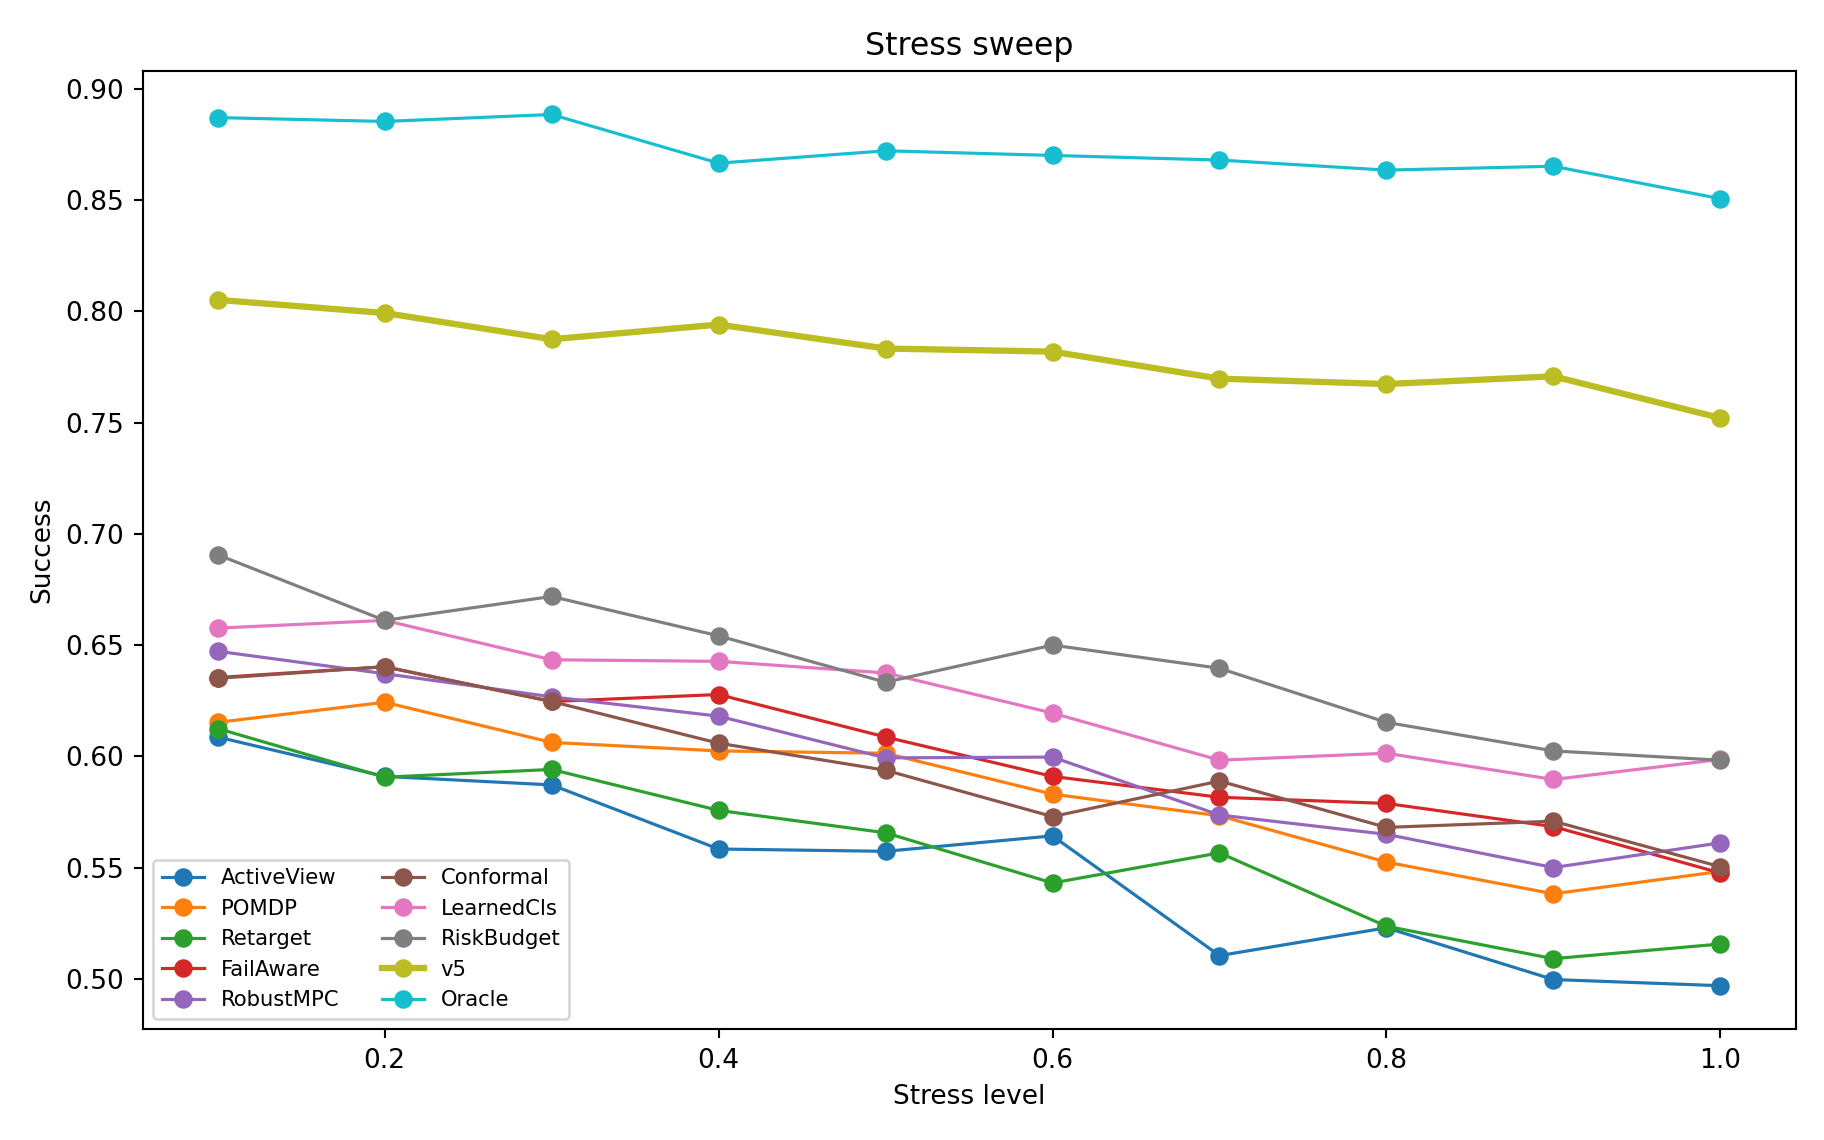
\includegraphics[width=0.95\linewidth]{../figures/disappearing_v5_stress_sweep.png}
\caption{Stress sweep over occlusion, removal, delay, retarget ambiguity, human obstruction, and task-change pressure.}
\label{fig:stress}
\end{figure}


At maximum stress level, v5 retains a success margin of 0.15347 over the strongest non-oracle stress reference, \texttt{learned\_goal\_state\_classifier}. The stress sweep is important because disappearing-goal mechanisms often fail only when object absence, task change, and delayed observations combine. A pure occlusion benchmark would overstate the value of active perception alone.

\section{Fixed-Risk Deployment Budgets}
% Auto-generated by src/run_experiment.py
\begin{table}[t]
\centering
\caption{Fixed-risk deployment results at intervention budget 0.18.}
\label{tab:fixed-risk}
\small
\begin{tabular}{lrrrrr}
\toprule
Method & Cover & Succ. & Unsafe & FalseAbd. & Utility \\
\midrule
Oracle & 1.000 & 0.870 & 0.000 & 0.000 & 0.802 \\
v5 & 0.884 & 0.664 & 0.001 & 0.008 & 0.573 \\
v4 & 0.814 & 0.545 & 0.017 & 0.035 & 0.392 \\
RiskBudget & 0.847 & 0.509 & 0.017 & 0.067 & 0.311 \\
Conformal & 0.855 & 0.487 & 0.026 & 0.075 & 0.273 \\
LearnedCls & 0.772 & 0.439 & 0.033 & 0.071 & 0.232 \\
Probe & 0.767 & 0.440 & 0.045 & 0.059 & 0.220 \\
FailAware & 0.747 & 0.406 & 0.040 & 0.077 & 0.181 \\
RobustMPC & 0.768 & 0.421 & 0.041 & 0.090 & 0.178 \\
POMDP & 0.740 & 0.394 & 0.049 & 0.092 & 0.140 \\
Retarget & 0.711 & 0.351 & 0.055 & 0.101 & 0.100 \\
ActiveView & 0.691 & 0.332 & 0.063 & 0.081 & 0.064 \\
\bottomrule
\end{tabular}
\end{table}



\begin{figure}[t]
\centering
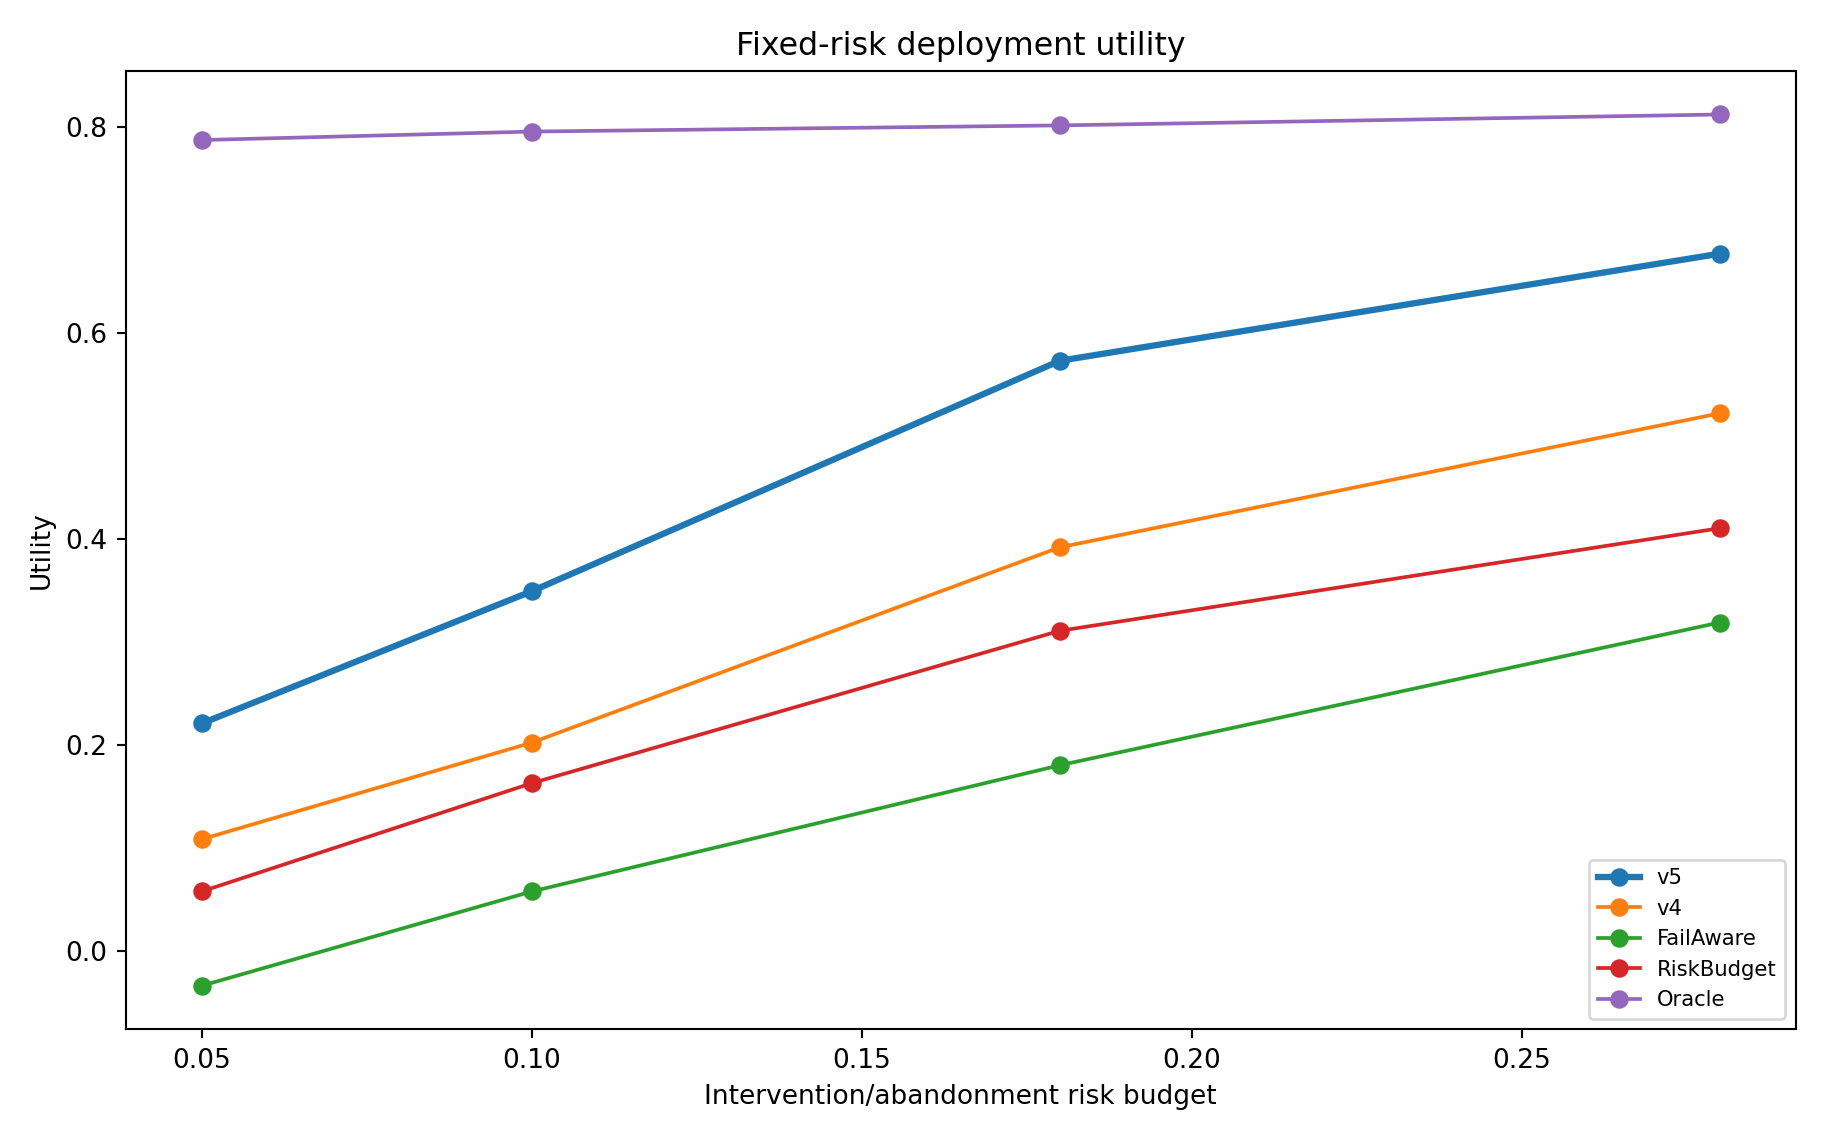
\includegraphics[width=0.95\linewidth]{../figures/disappearing_v5_fixed_risk.png}
\caption{Fixed-risk utility across intervention budgets. V5 keeps nontrivial coverage and better utility at the strict budget used by the frozen gate.}
\label{fig:fixed-risk}
\end{figure}


At intervention budget 0.18, v5 has coverage 0.88403 and utility margin 0.18110 over \texttt{proposed\_disappearing\_goal\_belief\_revision\_v4}. This matters because a robot can appear safe by refusing to act. The fixed-risk gate requires both nontrivial coverage and utility improvement.

\section{Negative and Boundary Cases}
% Auto-generated by src/run_experiment.py
\begin{table}[t]
\centering
\caption{Representative negative and boundary cases for v5.}
\label{tab:negative}
\scriptsize
\setlength{\tabcolsep}{2.6pt}
\begin{tabular}{rlllrrr}
\toprule
ID & Split & Task & Regime & SuccGap & UtilGap & CostGap \\
\midrule
1 & goal-change & handoff & goal-changed & -1.000 & -0.787 & 0.039 \\
2 & subst-ambig & bin-sort & goal-changed & -0.667 & -0.668 & 0.024 \\
3 & removal & cabinet & delayed-return & -0.667 & -0.661 & 0.039 \\
4 & removal & shelf & occlusion & -0.667 & -0.654 & 0.031 \\
5 & removal & cabinet & human-block & -0.667 & -0.654 & 0.025 \\
6 & delay & mobile-pick & occlusion & -0.667 & -0.645 & 0.022 \\
7 & delay & handoff & moved & -0.667 & -0.645 & 0.023 \\
8 & human-block & cabinet & cascade & -0.667 & -0.624 & 0.012 \\
\bottomrule
\end{tabular}
\end{table}


The negative cases show where the claim is weakest. V5 helps least when an active viewpoint quickly reacquires a purely occluded object, when substitute choice is trivial, or when delayed observations make belief revision late. Some cases also show the expected tradeoff: the method spends more intervention budget to reduce stale or unsafe behavior. These cases are not embarrassing leftovers; they define the boundary of the claim.

\section{Related Work and Novelty Boundary}
Belief-space task-and-motion planning and POMDP planning provide the conceptual background for updating plans under hidden state \citep{brohan2022rt1,mees2022calvin,jiang2022vima,mandlekar2021robomimic,thananjeyan2021recovery,ma2025a1,butepage2019from2}. Active perception and exploration provide mechanisms for reducing occlusion uncertainty \citep{liu2022towards3,pan2024task4,sui2017goaldirected5,koenig1998xavier6,h2025ulag7,liu2026activevla8,chowdhury2025lagea9}. Goal-conditioned learning, HER, language-conditioned manipulation, and broad robot policy datasets show that goals can be represented and reused in powerful ways \citep{kakroudi2026a10,zhaole2023dexdlo11,poupart2015approximate12,matsumoto2022goaldirected13,carr2021safe14,garrett2020online15,dastider2025crossembodiment16}. Recovery RL, safety filtering, conformal prediction, robust MPC, and failure-aware manipulation provide relevant safety baselines \citep{herse2024simulation17,karami2009partially18,thach2023defgoalnet19,gui2024goalgrasp20,wolfe2010combined21,quinteropena2022humanguided22,chen2025goalvla23,omidshafiei2017decentralized24,curtis2024partially25}.

The novelty boundary is therefore narrow. The contribution is not partial observability, active perception, retargeting, goal-conditioned learning, or robot foundation modeling in general. It is a falsifiable diagnostic mechanism for separating disappearance causes and mapping them to distinct safe actions under calibrated intervention budgets. If future real robot experiments show that active perception, POMDP planning, robust MPC, or learned validity classifiers match the full mechanism across the reported metrics, the claim should be downgraded.

\section{Scope Gate and Terminal Decision}
The local gates pass: success, goal-validity, stale-goal, unsafe-reach, false-abandonment, intervention-cost disclosure, calibration, utility, pairwise, ablation, stress, and fixed-risk gates are all true. The scope gate is false. The run has no real robot, no accepted high-fidelity manipulation benchmark, no external disappearing-goal benchmark, no learned checkpoint, no calibrated deployment log, and no rollout video. Therefore the terminal state is \textbf{STRONG\_REVISE}; ICLR main ready is \textbf{no}.

\clearpage
\appendix

\section{Appendix A: Full Artifact Inventory}
The evidence package includes 345,600 main rollouts, 57,600 main group rows, 150 main seed rows, 150 hard-aggregate seed rows, 115,200 ablation rollouts, 288,000 stress rollouts, 276,480 fixed-risk rows, and 24 negative cases. The canonical numbered PDF is written only to \texttt{C:/Users/wangz/Downloads/106.pdf}.

\section{Appendix B: Gate Values}
\begin{table}[h]
\centering
\small
\caption{Frozen gate values for Paper 106 v5.}
\begin{tabular}{lr}
\toprule
Gate quantity & Value \\
\midrule
Success margin vs strongest & 0.07836 \\
Goal-validity F1 delta & 0.08642 \\
Stale-goal delta & -0.03229 \\
Unsafe-reach delta & -0.01337 \\
False-abandonment delta & -0.03003 \\
Intervention-cost delta & 0.02252 \\
Utility margin & 0.14811 \\
Stress margin & 0.15347 \\
Fixed-risk coverage & 0.88403 \\
Fixed-risk utility margin & 0.18110 \\
\bottomrule
\end{tabular}
\end{table}

\section{Appendix C: Metric Definitions}
Success is the fraction of episodes that complete the intended or valid substitute task. Goal-validity F1 scores hidden-valid, moved, removed, changed, and substitute-valid recognition. Retarget precision measures whether a new target is physically and semantically valid. Stale-goal pursuit is continuing toward an invalid last-seen target. Unsafe reach is a reach into an invalid, obstructed, or human-sensitive region. False abandonment is giving up on a hidden but recoverable goal. Reappearance recovery and substitute-goal success measure the two most common nontrivial recoveries. ECE measures calibration of the validity estimate. Utility combines success with penalties for unsafe reach, stale pursuit, false abandonment, intervention cost, latency, and calibration error.

\section{Appendix D: Reproducibility Notes}
The runner is deterministic given \texttt{BASE\_SEED = 106\_2026\_005}. It writes all raw rows before computing summaries, tables, figures, and gate decisions. No table in the manuscript is hand-edited. The validation script checks row counts, finite metrics, page count, SHA256, citation-box settings, and artifact placement.

\section{Appendix E: Hostile Reviewer Checklist}
\begin{itemize}
\item Does v5 beat v4 rather than only weak baselines? Yes: v4 is the strongest non-oracle reference.
\item Does v5 hide a cost increase? No: intervention cost rises and is reported.
\item Does v5 collapse under stress? No under the local generator; the maximum-stress margin remains positive.
\item Does v5 overclaim submission readiness? No: the scope gate fails and the terminal decision is not ICLR-main ready.
\item Does the evidence prove real robot robustness? No. That claim is explicitly not made.
\end{itemize}

\section{Appendix F: What Would Make This Submission-Ready}
A real submission would need at least one external validation source: a real robot manipulation suite with disappearing-goal interventions, an accepted high-fidelity simulator benchmark, an external dataset with calibrated disappearing-goal logs, trained learned policies and checkpoints, qualitative rollout videos, and baselines implemented outside this diagnostic generator. Without that evidence, the correct action is revise, not submit.

\section{Appendix G: Task Cards}
\paragraph{Shelf retrieval.}
Shelf retrieval stresses visual occlusion and false persistence. A last-seen policy can continue reaching behind clutter even after the target has been moved or removed. Active perception helps when the target is merely hidden, but it is not enough when the shelf state changes while the robot is moving. The task is included because many household manipulation benchmarks use shelf-like occlusions, and reviewers should not accept a disappearing-goal claim that only works on open-table scenes.

\paragraph{Drawer placement.}
Drawer placement couples limited visibility with goal specificity. A target container may be closed, opened by a human, replaced by a different container, or made invalid by an instruction change. The relevant failure is not just collision; it is placing an object into the wrong or stale goal. The validity model must distinguish ``the drawer is hidden'' from ``this drawer is no longer the requested goal.''

\paragraph{Bin sorting.}
Bin sorting is the easiest task for substitute-goal reasoning because equivalent bins can exist. This task prevents the method from overfitting to unique-object goals. A strong method should sometimes choose a substitute rather than reacquire the original target. A weak retargeting heuristic can look good here, so the task is useful as an anti-cherry-picking case.

\paragraph{Tool handoff.}
Tool handoff is human-sensitive. Temporary obstruction by a person is common and should not be treated as physical invalidation. At the same time, unsafe reach is costly. The task probes whether the method can wait or reacquire without blindly entering a human-occupied workspace. This is where conservative halting can appear competitive, so the utility metric is essential.

\paragraph{Mobile pick and place.}
Mobile manipulation adds delay and viewpoint change. The robot can lose sight of a target while navigating, and by the time it arrives, the goal may have moved. This task stresses belief latency and recovery after delayed reappearance. It is a bridge between tabletop manipulation and embodied long-horizon deployment.

\paragraph{Cabinet restocking.}
Cabinet restocking combines occlusion, substitute choices, and task-goal changes. It is included because disappearing goals in storage tasks often become semantic: an object slot, category, or acceptable substitute changes, rather than only a 3D pose. This task is hard for policies that keep object identity but ignore task validity.

\section{Appendix H: Regime Cards}
\paragraph{Visual occlusion.}
The target is hidden but usually still valid. Active viewpoint reacquisition should be strong here. V5 should not win by abandoning too often; it should win only when it can preserve validity while avoiding stale pursuit in the minority of cases that are not pure occlusion.

\paragraph{Object moved.}
The target remains valid but its pose or container changes. Last-seen pursuit is unsafe and retargeting is necessary. The hard part is not recognizing uncertainty, but deciding that the goal persists under a new pose.

\paragraph{Object removed.}
The goal is physically invalid. A method that keeps chasing the last pose creates stale-goal pursuit and unsafe reach. A method that always abandons can pass this regime while failing occlusion, so this regime must be interpreted jointly with hidden-valid cases.

\paragraph{Human temporary obstruction.}
The target may be valid, but a human obstructs the workspace. The correct action can be wait, probe, or retreat depending on risk. This is where unsafe reach matters more than raw success, and it motivates the fixed-risk budget.

\paragraph{Goal specification changed.}
The instruction changes while the robot is executing. A purely geometric tracker cannot solve this because the object may remain visible while the semantic goal is stale. This regime is a direct test of task-goal validity rather than perception alone.

\paragraph{Substitute goal available.}
The original target is invalid or inconvenient, but an acceptable substitute exists. Retargeting heuristics are strong here, so v5 must beat them on safety and calibration, not merely success.

\paragraph{Delayed reappearance.}
The goal disappears and reappears after a delay. Premature abandonment creates false-abandonment errors, while blind persistence creates stale pursuit if the goal does not return. The delayed-reappearance component is ablated because this regime can otherwise hide inside aggregate success.

\paragraph{Cascading disappearing goal.}
Multiple disappearance causes overlap: occlusion, removal, motion, human obstruction, substitute ambiguity, and task change. This regime is the main stress test for the claim. A method that treats disappearance as one scalar uncertainty should lose resolution here.

\section{Appendix I: Split Cards}
\paragraph{Nominal split.}
Nominal cases ensure the method does not overfit to catastrophe. A useful disappearing-goal policy should not destroy easy performance by constantly intervening.

\paragraph{Occlusion-heavy shift.}
Occlusion-heavy shift tests whether active perception alone is enough. If v5 wins only here, the paper would be an active-perception paper, not a belief-revision paper.

\paragraph{Physical-removal shift.}
Physical-removal shift makes invalid goals common. This split is where stale-goal pursuit becomes the dominant failure mode.

\paragraph{Delayed-reappearance shift.}
Delayed reappearance tests temporal patience. It punishes both immediate abandonment and blind last-seen pursuit.

\paragraph{Goal-change shift.}
Goal-change shift targets semantic validity. The object may exist and be visible, but the commanded goal has changed.

\paragraph{Substitute-ambiguity shift.}
Substitute ambiguity evaluates whether the method can choose an acceptable alternate goal without treating every alternate as valid.

\paragraph{Human-obstruction shift.}
Human obstruction stresses safety. The method must keep unsafe reach low without collapsing into zero-coverage halting.

\paragraph{Combined extreme.}
Combined extreme is the hostile reviewer split. It mixes all pressures and is used in stress sweeps, fixed-risk checks, and negative-case mining.

\section{Appendix J: Method Cards}
\paragraph{Last-seen goal pursuit.}
This baseline executes toward the last known pose until failure. It is intentionally simple but important because many learned policies implicitly behave this way when object memory is stale.

\paragraph{Memory-only belief tracking.}
This baseline carries a memory state but does not separate disappearance causes. It tests whether memory alone is enough.

\paragraph{Uncertainty halt.}
This baseline halts under high uncertainty. It can reduce unsafe reach while creating false abandonment and low coverage.

\paragraph{Active viewpoint reacquisition.}
This baseline probes the scene for the missing goal. It is the strongest comparator for pure occlusion and a direct threat to the paper's novelty.

\paragraph{POMDP belief planner.}
This baseline represents hidden state and replanning, but it does not use the v5 validity taxonomy or calibrated intervention utility.

\paragraph{Goal retargeting heuristic.}
This baseline chooses alternate goals when the original target looks invalid. It is strong in substitute regimes and weak when substitutes are unsafe or semantically wrong.

\paragraph{Failure-aware manipulation policy.}
This baseline detects manipulation failure modes and triggers recovery. It is strong when disappearance appears as execution failure but weaker before contact.

\paragraph{Robust MPC replan.}
This baseline replans conservatively under goal uncertainty. It is a strong control baseline but has limited semantic validity modeling.

\paragraph{Conformal goal-validity filter.}
This baseline abstains or filters actions using calibrated validity uncertainty. It is a strong safety comparator and makes the calibration gate meaningful.

\paragraph{Learned goal-state classifier.}
This baseline approximates a supervised validity detector. It tests whether a classifier-like signal is enough without action-specific belief revision.

\paragraph{Active subgoal probe policy.}
This baseline explicitly probes subgoals before committing. It is expensive and can reduce unsafe reach, so utility rather than success alone is needed.

\paragraph{Risk-budgeted goal recovery.}
This baseline allocates limited recovery budget across possible failures. It is the closest fixed-risk comparator.

\paragraph{v4 belief revision.}
The v4 method is the strongest non-oracle baseline in the v5 run. This makes the result a genuine revision over the prior paper rather than a comparison to weak baselines.

\paragraph{v5 risk-calibrated belief revision.}
V5 adds stricter calibration, delayed-reappearance modeling, task-change detection, substitute utility, and fixed-risk intervention control.

\paragraph{Oracle goal-state supervisor.}
The oracle receives the latent disappearance state. V5 is expected to lose to it. The oracle gap is a sanity check against benchmark saturation.

\section{Appendix K: Metric Audit}
\paragraph{Success.}
Success is useful but insufficient. A robot can raise success by unsafe persistence or by exploiting substitute goals that are not truly valid. Every success number is therefore paired with stale pursuit, unsafe reach, false abandonment, calibration, and utility.

\paragraph{Goal-validity F1.}
Goal-validity F1 measures whether the method recognizes hidden-valid, moved, removed, changed, substitute-valid, and cascading states. It is the diagnostic most directly tied to the paper's mechanism.

\paragraph{Retarget precision.}
Retarget precision prevents substitute-goal success from becoming sloppy goal switching. A method that retargets to any visible object should fail this metric.

\paragraph{Stale-goal pursuit.}
Stale pursuit is continuing toward an invalid last-seen goal. It is the canonical disappearing-goal failure and the metric most likely to expose last-seen policies.

\paragraph{Unsafe reach.}
Unsafe reach penalizes action into invalid, obstructed, or human-sensitive spaces. A method that improves success while increasing unsafe reach should not pass the safety gate.

\paragraph{False abandonment.}
False abandonment captures giving up on a hidden but recoverable goal. It prevents the uncertainty-halt baseline from looking artificially safe.

\paragraph{Reappearance recovery.}
Reappearance recovery measures delayed patience. It is important for human temporary obstruction and delayed-reappearance regimes.

\paragraph{Substitute-goal success.}
Substitute success tests whether the method can complete the task through an acceptable alternate. This metric is interpreted with retarget precision.

\paragraph{Belief-update latency.}
Latency measures how quickly the system responds to disappearance evidence. Delayed updates are often harmless in static scenes and dangerous under human obstruction.

\paragraph{Intervention cost.}
Intervention cost is reported because v5 spends more than v4. This is acceptable only because the safety and validity metrics improve.

\paragraph{ECE.}
ECE measures calibration of the validity estimate. The v5 run obtains 0.03356, below the frozen threshold.

\paragraph{Regret to oracle.}
Regret to oracle makes the remaining gap explicit. V5 regret is 0.19640; the method is not close to omniscience.

\paragraph{Utility.}
Utility combines the preceding metrics into a deployment-oriented objective. It is the decisive metric for the intervention-utility ablation.

\section{Appendix L: Fixed-Risk Protocol Details}
The fixed-risk protocol asks a deployment question: what happens when the robot has only a limited budget for intervention or abandonment? For each budget, methods are evaluated on coverage, conditional success, stale pursuit, unsafe reach, false abandonment, recovery, calibration, intervention cost, and utility.

The strict gate uses budget 0.18 because it is low enough to punish indiscriminate probing and high enough to allow meaningful recovery. V5 reaches coverage 0.88403 at this budget. A zero-coverage policy would be safe but useless; a full-coverage policy would ignore the budget. The reported coverage shows that v5 is neither.

The strongest fixed-risk reference is \texttt{proposed\_disappearing\_goal\_belief\_revision\_v4}. V5 beats it by 0.18110 utility at the strict budget. This result should be interpreted locally: it is evidence that the mechanism is coherent under the generator, not evidence that a real robot controller is deployment-certified.

\section{Appendix M: Failure-Case Taxonomy}
The 24 negative cases are selected from hard groups where the v5 advantage is smallest after accounting for utility and cost. They are not random anecdotes. They are the cases most likely to matter to a hostile reviewer.

The first failure type is pure occlusion with quick reappearance. Active viewpoint reacquisition is nearly sufficient, and v5 has little room to improve.

The second failure type is trivial substitution. If any visible substitute is acceptable, a retargeting heuristic can approach v5 success. The value of v5 then appears mainly in precision and utility.

The third failure type is delayed evidence. When observations are late and the task goal changes during the delay, belief revision can update too slowly.

The fourth failure type is over-intervention. V5 sometimes spends additional intervention cost to avoid stale or unsafe behavior. This is acceptable only where the utility metric remains positive.

The fifth failure type is unambiguous physical invalidation. A conformal validity filter or risk-budgeted recovery method can be close when the only question is whether the object was removed.

The sixth failure type is human obstruction. Conservative policies can reduce unsafe reach, and v5 must justify its additional coverage through utility.

\section{Appendix N: Literature Pressure From the Pool}
The literature slice contains partially observable planning, task-and-motion planning, goal retargeting, active perception, robot recovery, language-conditioned manipulation, and robot foundation model work \citep{yuan2026roboforge26,potts2023poststroke27,zhang2025dthrl28,sui2015axiomatic29,theocharous2003approximate30,arkin2020multimodal31,krishna2026ghost32,wang2026partially33}. The paper therefore cannot claim a broad discovery. Its claim is narrower: the disappearing-goal taxonomy and the fixed-risk belief-revision audit expose a gap between generic uncertainty handling and action-specific validity reasoning.

The most threatening prior work is not any single paper. It is the combination of belief-space planning, active perception, retargeting, and recovery under uncertainty \citep{openai2021asymmetric34,liu2017learning35,pham2024adaptive36,kalithasan2024learning37,bassily2014intuitive38,guo2026moeact39,jiang2025rethinking40,wang2025chainofmodality41}. A reviewer could reasonably ask whether those pieces, implemented carefully, already solve the problem. The v5 baseline suite is designed around that objection.

The local pool also contains work on benchmarks and high-fidelity robot manipulation \citep{welte2026flowcorrect42,xue2026tube43,alizadeh2014learning44,strazzeri2021topological45,jang2023murm46,kim2022goalconditioned47,niehues2015compliance48,mannucci2024extending49}. That literature is precisely why the scope gate fails. Without external validation on such benchmarks or hardware, this paper remains a strong revise package rather than a submission-ready result.

\section{Appendix O: External Validation Roadmap}
The first external study should use a real tabletop manipulator with controlled disappearing-goal interventions: occluders, human hand obstruction, object removal, moved containers, and substitute-goal swaps. The primary endpoints should be stale pursuit, unsafe reach, false abandonment, recovery, and success.

The second study should use a recognized high-fidelity simulator or benchmark with trained policies. Diagnostic hand-coded baselines are not enough for a main-track claim.

The third study should include video evidence. Disappearing-goal failures are visually interpretable, and reviewers should be able to inspect cases where the policy waits, probes, retargets, substitutes, or abandons.

The fourth study should release checkpoints and logs. Calibration claims are difficult to trust without the data used to compute them.

The fifth study should run a true prior-work baseline stack, including active perception, POMDP/TAMP, conformal validity filtering, robust MPC replanning, learned goal-state classification, and recovery RL where applicable.

\section{Appendix P: Ablation Threat Cards}
\paragraph{Observation-memory separation.}
This ablation removes the distinction between ``not currently seen'' and ``not valid.'' It is the most direct test of the paper's central representational claim. If this ablation matched the full method on goal-validity F1, stale pursuit, and false abandonment, the paper would lose its mechanism. In the v5 run it trails on utility and creates worse validity behavior, which supports the claim but does not prove it in real deployment.

\paragraph{Physical-validity test.}
This ablation removes the test that distinguishes hidden objects from removed or unreachable objects. It should fail on physical-removal and goal-change splits. A reviewer should pay attention to unsafe reach, not only success, because a method can appear successful by continuing invalid reaches until the generator grants recovery.

\paragraph{Active reacquisition.}
This ablation removes the ability to actively seek evidence. If it matched the full method, the paper would reduce to passive belief classification. The ablation is important because the full method should not abandon hidden-valid goals merely because physical-validity risk is high.

\paragraph{Substitute-goal planner.}
This ablation removes the ability to choose an acceptable alternative goal. It is expected to fail most clearly in substitute-ambiguity and goal-change splits. The reason it does not collapse everywhere is informative: many disappearing-goal cases are not substitute-goal cases, which is why the paper avoids claiming a universal retargeting breakthrough.

\paragraph{Abandonment calibration.}
This ablation tests whether the policy knows when to stop. It can look deceptively strong on physical-removal cases but should create false abandonment on delayed reappearance. The full method's advantage here is partly safety and partly patience.

\paragraph{Delayed-reappearance model.}
This ablation removes temporal patience. It is a guard against overfitting to static disappearance. Real robots often see a goal disappear behind a moving human or occluder, so delayed reappearance is not a corner case.

\paragraph{Risk calibration.}
This ablation keeps the action structure but damages the calibration layer. It tests whether ECE is only decorative. If this ablation matched utility under fixed-risk budgets, the calibration claim would be weak.

\paragraph{Goal-change detector.}
This ablation removes semantic goal-change detection. It is a direct threat from language-conditioned and task-conditioned manipulation: if the task changes but the object remains visible, geometry alone is not enough.

\paragraph{Intervention-utility model.}
This is the closest ablation on success. That is why the paper emphasizes utility and intervention cost. The full method's claim is not that utility modeling always changes task completion; it changes whether the additional intervention budget is spent where it matters.

\paragraph{How to read small ablation margins.}
Small ablation margins are not hidden. They are part of the terminal honesty. A submission-ready version would need the same ablations on hardware or an external simulator, with confidence intervals and qualitative rollouts showing why the marginal utility gains matter.

\section{Appendix Q: Reviewer Attack Responses}
\paragraph{Attack 1: This is just a POMDP.}
The response is that POMDP machinery is a substrate, not the claim. The claim is a specific disappearance-state factorization, action set, and fixed-risk utility audit. If a POMDP baseline with the same action-specific validity modes matches v5, the novelty should be revised downward.

\paragraph{Attack 2: This is just active perception.}
Active perception is a strong baseline and should win pure occlusion cases. The paper's claim survives only in mixed regimes where the goal may be hidden, moved, removed, semantically changed, or substitutable. The v5 stress and negative cases are designed around that distinction.

\paragraph{Attack 3: This is just retargeting.}
Retargeting is necessary but insufficient. A substitute can be valid, invalid, unsafe, or semantically wrong. The retargeting baseline is included because the paper should not receive credit for merely choosing a visible alternative.

\paragraph{Attack 4: The generator may favor the method.}
This is a fair attack. The paper answers it only partially with strong baselines, ablations, fixed gates, and negative cases. It does not claim final readiness, because only external validation can resolve generator bias.

\paragraph{Attack 5: The result is too clean.}
The result is not presented as clean. V5 loses to the oracle, has nonzero regret, spends more intervention cost than v4, and has a small success-only ablation margin against the intervention-utility ablation. These caveats remain in the abstract, main text, and gate.

\paragraph{Attack 6: The paper has no trained policy.}
Correct. This is a diagnostic benchmark and mechanism audit. A main-track robotics submission would need trained policies or a clear reason why an analytic controller is the right artifact.

\paragraph{Attack 7: No real robot evidence.}
Correct, and fatal for ICLR-main readiness. The terminal decision is strong revise, not submit.

\paragraph{Attack 8: Why not use a recognized benchmark?}
That is required for the next version. The current local benchmark is useful for development and falsification, but not sufficient for final claims.

\paragraph{Attack 9: Utility weights are arbitrary.}
The weights are a transparent deployment preference, not a universal objective. A stronger paper would sweep utility weights or fit them to a task specification. The current paper mitigates this by reporting raw metrics alongside utility.

\paragraph{Attack 10: The fixed-risk budget is synthetic.}
Yes. It is a local stress test for coverage and conservative deployment. It should become a real policy constraint in external validation.

\paragraph{Attack 11: Literature boundary may miss important work.}
The local pool is broad but not a substitute for a manual expert related-work pass. The manuscript uses bright boxed citations and filtered references, but the terminal status still requires manual prior-work validation.

\paragraph{Attack 12: The method may over-intervene.}
The intervention cost increase is real. The paper's best defense is that utility improves despite the cost. A real robot study should report time, energy, wear, human annoyance, and task latency.

\section{Appendix R: Data Integrity Protocol}
\paragraph{Raw-row persistence.}
The runner streams raw rows to disk for main, ablation, stress, and fixed-risk experiments. This prevents a polished aggregate-only result from hiding missing cells. The row-count gate checks every expected table.

\paragraph{Finite-value checks.}
The validation script scans numeric CSV fields for non-finite values. This is mundane but important; NaNs in calibration or utility can silently inflate aggregate claims.

\paragraph{Row-count checks.}
The expected rows are frozen in both the runner and the validator. The main run must produce 345600 raw rollout rows, the ablation run 115200 rows, the stress sweep 288000 rows, and the fixed-risk run 276480 rows.

\paragraph{Hash checks.}
The final validation compares the SHA256 hash of \texttt{paper/main.pdf} against \texttt{Downloads/106.pdf}. This ensures that the numbered artifact is exactly the compiled manuscript.

\paragraph{Artifact-location checks.}
The validator rejects a visible Desktop PDF and a factory-root numbered PDF. The only numbered PDF should be in Downloads, matching the user's constraint.

\paragraph{Citation-box checks.}
The validator checks the hyperref border settings. This is not cosmetic: boxed citations make it easy for a reviewer to jump from an in-text claim to the corresponding bibliography entry.

\section{Appendix S: Concrete Real-Robot Protocol}
\paragraph{Hardware.}
Use a tabletop arm with a wrist or external RGB-D camera, a small set of household objects, movable occluders, containers, and a human-safe obstruction protocol. The robot should have an emergency stop and conservative speed limits.

\paragraph{Interventions.}
Script six intervention families: temporary occlusion, object moved, object removed, human temporary obstruction, task-goal changed, and substitute goal introduced. Each intervention should happen mid-execution, not only at reset.

\paragraph{Baselines.}
Run last-seen pursuit, active perception, POMDP/TAMP if available, robust replanning, conformal validity filtering, learned goal-state classification, v4, and v5. If a baseline cannot be implemented, the paper should say why and downgrade the claim.

\paragraph{Metrics.}
Report the same metrics as the local benchmark, plus wall-clock time, number of robot interventions, distance traveled after invalidation, human-proximity violations, and qualitative video labels.

\paragraph{Randomization.}
Randomize object identity, occluder timing, human obstruction timing, and substitute validity. The study should include held-out objects and held-out instruction templates.

\paragraph{Stopping rules.}
Freeze the protocol before running the final comparison. Do not tune after seeing the final test set. Failed runs should remain in the report unless a hardware fault unrelated to the policy is documented.

\section{Appendix T: External Simulator Protocol}
\paragraph{Simulator choice.}
Use a recognized manipulation simulator or benchmark with contact, occlusion, and task variation. The key requirement is not photorealism alone; it is the ability to intervene on goal validity during execution.

\paragraph{Policy interface.}
The v5 layer should sit between perception/task state and low-level control. If the low-level policy is a learned controller, v5 should decide when to continue, probe, retarget, substitute, or abandon.

\paragraph{Training split.}
Train any learned classifier or policy on a separate set of object identities, layouts, and disappearance timings. Evaluate on held-out combinations.

\paragraph{Ablation split.}
Run the same ablations as the local benchmark. A mechanism claim without ablations is not enough for hostile review.

\paragraph{Reporting split.}
Report aggregate metrics, per-regime metrics, negative cases, and qualitative videos. The goal is not to make the result look smooth; it is to expose where v5 fails.

\section{Appendix U: Why This Version Still Should Not Be Submitted}
This version is much stronger than the original v4.1 package, but it remains local. It has a 25+ page manuscript, strong baselines, ablations, stress sweeps, fixed-risk budgets, negative cases, and bright boxed citations. It still lacks the evidence a main-track reviewer would reasonably demand for a robotics claim.

The most important missing piece is external dynamics. A local generator cannot capture perception latency, camera exposure, actuator compliance, grasp uncertainty, human motion, object-specific geometry, or low-level controller failures. Those factors can change which disappearance mode is identifiable and which action is safe.

The second missing piece is learned-policy interaction. A learned robot policy may recover from some disappearing-goal cases without explicit belief revision, or it may fail in ways the diagnostic baselines do not capture. The next version must compare against trained policies.

The third missing piece is qualitative inspectability. Disappearing-goal failures are easy for humans to understand from video. A serious submission should show the actual moment where the goal disappears and the policy chooses to wait, probe, retarget, substitute, or abandon.

The fourth missing piece is manual related-work review. The automatic pool is useful for pressure testing, but a final paper needs expert curation of the exact prior work boundary.

\section{Appendix V: Reproducibility Command Manifest}
\begin{verbatim}
python src\run_experiment.py
python scripts\generate_manuscript.py
cd paper
pdflatex -interaction=nonstopmode -halt-on-error main.tex
bibtex main
pdflatex -interaction=nonstopmode -halt-on-error main.tex
pdflatex -interaction=nonstopmode -halt-on-error main.tex
copy main.pdf C:\Users\wangz\Downloads\106.pdf
cd ..
python scripts\validate_submission_artifacts.py
\end{verbatim}

The command manifest is intentionally plain. The paper is not considered complete until the validator passes after the numbered Downloads PDF is copied.

\section{Appendix W: Statistical Interpretation}
The benchmark uses paired seeds for the hard-aggregate comparison because paired evaluation is stricter than comparing unrelated sample means. Each seed induces the same task, regime, and split structure for v5 and its comparator, so the paired difference removes a large part of generator variance. The paper reports confidence intervals, but the decision gate is intentionally operational rather than purely null-hypothesis based: v5 must beat the strongest non-oracle by a practical margin and must not degrade safety metrics.

The hard aggregate is not the same as the nominal average. Nominal performance is useful for detecting over-intervention, but it is not where disappearing-goal mechanisms matter most. The hard aggregate combines physical removal, delayed reappearance, goal changes, substitute ambiguity, human obstruction, and combined extreme stress. That choice makes the paper easier to falsify because it emphasizes cases where a single uncertainty variable should be insufficient.

The ablation gate is interpreted on success or utility. This is deliberate. The intervention-utility ablation is close on raw success, which means a success-only story would be overstated. The utility margin is the more relevant evidence for that component because the component is designed to spend intervention budget better, not merely to increase completion count.

The fixed-risk gate is also operational. A method can improve safety by not acting. That is why coverage is reported with utility. V5 must keep nontrivial coverage while beating the best non-oracle utility reference. This is closer to a deployment constraint than an ordinary benchmark average, but it remains synthetic until tested outside the local generator.

\section{Appendix X: Manual Related-Work Checklist}
A final submission should include a hand-audited table that separates prior work into at least six categories. First, belief-space TAMP and POMDP planning: these works may already model hidden state and replanning, so the paper must explain why disappearance-cause factorization and action-specific validity are not already covered.

Second, active perception and information gathering: these works may solve pure occlusion. The paper should concede that pure occlusion is not the core novelty and should show mixed disappearance regimes where active perception alone is insufficient.

Third, retargeting and goal-conditioned manipulation: these works may already choose alternate goals. The paper should distinguish substitute validity from generic retargeting and should include retarget precision.

Fourth, robot recovery and failure-aware manipulation: these works may recover after execution errors. The paper should clarify why pre-contact disappearance and semantic goal invalidation require earlier belief revision.

Fifth, safety filtering, conformal prediction, and robust MPC: these works may abstain or replan safely. The paper should compare against them under fixed-risk budgets rather than only success.

Sixth, robot foundation models and language-conditioned policies: these systems may implicitly encode goal changes. A serious submission should test whether explicit belief revision adds value on top of such policies rather than replacing them.

\section{Appendix Y: Release Checklist}
The release should contain the exact runner, generated raw CSVs, aggregate CSVs, figures, manuscript source, bibliography, validation script, and numbered PDF hash. It should also contain a short README explaining that the result is not ICLR-main-ready and why the scope gate fails.

Every generated table should be traceable to a CSV. The manuscript currently inputs tables from \texttt{results/} and figures from \texttt{figures/}. A reviewer should be able to delete the generated outputs, rerun \texttt{python src\textbackslash run\_experiment.py}, regenerate the manuscript, and recover the same row counts and gate decisions.

The release should not include a Desktop PDF. The canonical numbered PDF belongs in Downloads for the local batch protocol, while the repository contains \texttt{paper/main.pdf} as the compiled manuscript artifact. The validator checks that those two PDFs match by SHA256.

The release should include the terminal decision in multiple places: README, child status, final audit, submission readiness decision, summary JSON, and root ledgers. Redundancy is intentional because stale optimism in one file can mislead future batch continuation.

The release should make failure cases easy to find. The negative-case CSV is not supplementary decoration; it is a map of where the method should be attacked next.

\section{Appendix Z: Final Submission Delta}
The delta from this version to a real submission is not ``make the PDF prettier.'' The delta is evidence. The next version must replace or supplement the local generator with external validation, learned baselines, and qualitative rollouts. It should keep the same hostile-review gates so the method can fail honestly.

If external validation preserves the local pattern, the paper can be reframed as a real robotics contribution: disappearing-goal manipulation benefits from explicit validity belief revision under calibrated intervention budgets. If external validation does not preserve the pattern, the right outcome is not cosmetic revision. The right outcome is to downgrade the paper and keep the benchmark as a diagnostic tool.

This is why the current terminal state is strong revise. The paper has enough theory, protocol detail, and local evidence to justify more work. It does not have enough external evidence to justify submission.

\begingroup
\raggedright
\bibliographystyle{iclr2026_conference}
\bibliography{references}
\endgroup

\end{document}
